%------------------------------- CHAPTER NAME --------------------------------
\chapter{Specific Range}
In this chapter an anlysis of the specific range is performed with the aim of obtain useful information about cruise performance. 

In particular, starting from generalized performance evaluation and interfacing them with the fuel consumption, the final objective will be to define the specific range as function of Mach number, obtaining the so called \emph{cruise grid chart} which is a very important tool for pilots because it allows to choose the correct speed, during cruising phase, in order to follow some mission objectives like minimum fuel consumption or a fast cruise.

%-------------------------- THEORETICAL BACKGROUND ---------------------------
\section{Theoretical background}
The first step that has to be done in order to obtain the \emph{cruise grid chart} is to define generalized performance in terms of thrust and drag. The \emph{generalized} attribute given to these quantities stands for the fact that they are independents from altitude and this result is reached through the parameter $\delta$ which represents a ratio between the total pressure at compressor inlet and  the standard pressure at sea level. 

\bigskip
\noindent
Regarding the thrust, the generalized version can be obtained by dividing it by $\delta$ as shown below.
\begin{eqnarray}
\frac{T}{\delta}=\frac{T_{f}}{\delta}-M\cdot a_{0}\cdot \frac{\sqrt{\theta \cdot m_{a}}}{\delta}
\label{eqn:Equation1}
\end{eqnarray}

\begin{figure}[!ht]
\centering
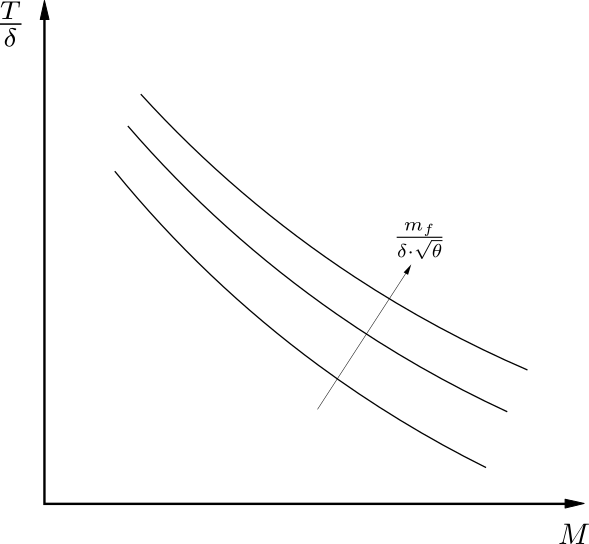
\includegraphics[keepaspectratio, width=0.50\textwidth]{TDelta}
\caption{Qualitative trend of  the generalized thrust v.s. Mach number parameterized in generalized fuel flow rate}
\label{fig:Figure1}
\end{figure}

\noindent
where

\begin{itemize}
\item $T$, is the net thust
\item $T_{f}$, is the gross thrust
\item $M$, is the mach number
\item $a_{0}$, is the sound speed at sea level
\item $\dfrac{\sqrt{\theta \cdot m_{a}}}{\delta}$, is the genralized air flow rate which is function of the generalized fuel flow rate given by $\dfrac{m_{f}}{\delta \cdot \sqrt{\theta}}$
\end{itemize}

\noindent
so that the genralized thrust results as a function of Mach number and generalized fuel flow rate.

\begin{eqnarray}
\frac{T}{\delta}=\frac{T_{f}}{\delta}\cdot f\left(\frac{m_{f}}{\delta \cdot \sqrt{\theta}}\right)
\label{eqn:Equation2}
\end{eqnarray}

\noindent
As shown in figure~\ref{fig:Figure1} the generalized thrust decreases with Mach number, at given fuel flow rate, and grows with the latter, at given Mach number. This because if the Mach number grows at fixed fuel flow rate, the air flow rate grows reducing the thrust; otherwise, if fuel flow rate grows at fixed Mach number, air flow rate is lower giving more thrust.

With this function it's possible to correlate generalized thrust to hourly fuel consumption which is a main keypoint in building the cruise grid chart of an endurance based aircraft such as UAV. 

Since transport aircrafts rely more on range performance, it's necessary to obtain the same relationship between generalized thurst and fuel consumption referred to the generalized specific range indicated with $\delta\bar s $. 

\bigskip
\noindent
Dividing the generalized fuel flow rate, which is dimesionally equal to $\frac{\si{\kilogram}}{\second}$, by a velocity, the result has a dimension of $\frac{\meter}{\si{\kilogram}}$ that represents the reciprocal of the specific range. In this way it's possible to state the following relation.

\begin{eqnarray}
\frac{m_{f}}{\delta \cdot \sqrt{\theta}}=\frac{M\cdot a_{0}}{\delta\bar s}
\label{eqn:Equation3}
\end{eqnarray}

\begin{figure}[!ht]
\centering
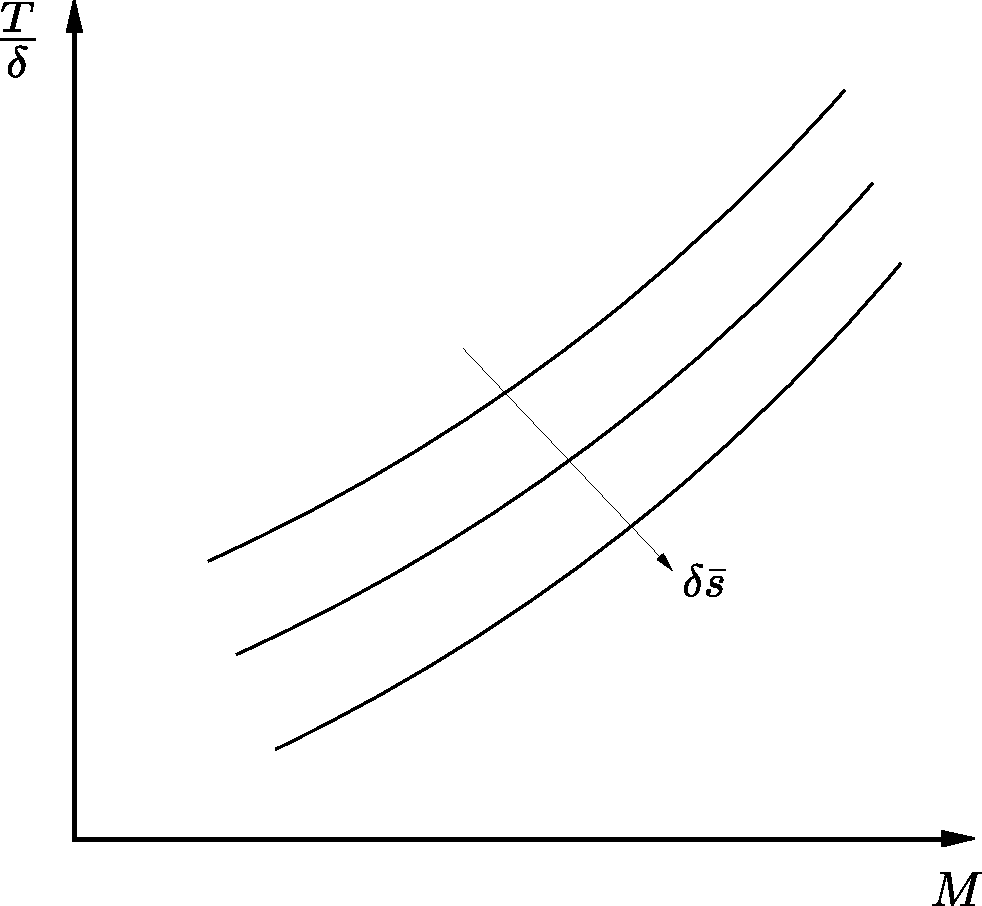
\includegraphics[keepaspectratio, width=0.50\textwidth]{TDelta_SpecificRange}
\caption{Qualitative trend of the generalized thrust v.s. Mach number parameterized in generalized specific range}
\label{fig:Figure2}
\end{figure}

\noindent
As expectd from the relation~\ref{eqn:Equation3} the thrust has a trend which is the inverse of the previous parameterization. In fact now, for a given Mach number, if the pilot wants to go farther he has to decrease the thrust in order to reduce the fuel consumption; otherwise, at a given distance to reach, the pilot has to increase the thrust in order to make the Mach number grows.

\bigskip
\noindent
Since the thrust has always to be compared with the drag in order to evaluate if the aircraft can fly in a specific cruise condition without loosing speed and altitude, it's necessary to obtain a generalized drag trend as well. 

This ai very similar to the drag trend, as can be seen from figure~\ref{fig:Figure3}, and it depends from aircraft weight as well; but, since these have to be generalized quantities, the weight is a generalized weight too.

\begin{figure}[b]
\centering
\includegraphics[keepaspectratio, width=0.50\textwidth]{DragDelta_SpecificRange}
\caption{Qualitative trend of the generalized drag v.s. Mach number parameterized in generalized weight}
\label{fig:Figure3}
\end{figure}

\bigskip
\noindent
By the overlap of figure~\ref{fig:Figure2} and figure~\ref{fig:Figure3} charts, it's easy to note that the best Mach number, for a given generalized weight, is located at the intersection of the two curves as reported in figure~\ref{fig:Figure4}. In fact, in order to obtain a bigger specific range at fixed weight, the generalized drag would be higher than the generalized thrust; otherwise, if the pilot wants to fly faster at given weight, he has to increase thrust so that the specific range will decrease due to the increasing fuel consumption.

Since during the cruise phase the aircraft weight decreases continuously, the pilot has to gain altitude in order to leave the generalized weight unchanged; this explains why during cruise the aircraft continues to climb. 

\begin{figure}[t]
\centering
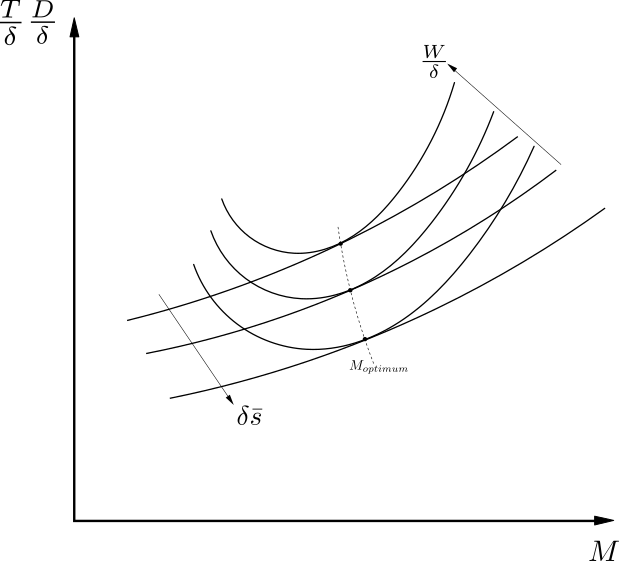
\includegraphics[keepaspectratio, width=0.50\textwidth]{TDeltaDragDelta}
\caption{Comparison between generalized drag and generalized thrust as functions of Mach number}
\label{fig:Figure4}
\end{figure}

\bigskip
\noindent
The specific range can also be connected to Breguet formulas, reported at~\ref{eqn:BreguetEquation1.1} and ~\ref{eqn:BreguetEquation1.2}, as it can be obtained by dividng the autonomy factor, $A.F.$, by the aircraft weight; in particular the autonomy factor, groups three main aircraft efficiency and can be written as follow.

\begin{eqnarray}
A.F.=\frac{\eta_{p}}{SFC}\cdot\frac{L}{D} %
\qquad \textrm {\parbox[t][][t]{.25\linewidth} {propeller aircraft}}
\label{eqn:A.F.Equation4}
\end{eqnarray}

\begin{eqnarray}
A.F.=\frac{V}{SFCJ}\cdot\frac{L}{D} %
\qquad \textrm {\parbox[t][][t]{.25\linewidth} {jet aircraft}}
\label{eqn:A.F.Equation5}
\end{eqnarray}

\noindent
where

\begin{itemize}
\item $\eta_{p}$, is propeller efficiency
\item $SFC$, is related to propulsive efficiency
\item $\frac{L}{D}$, is the aerodynamic efficiency
\end{itemize}

\noindent 
At given generalized weight and generalized specific range, the optimum Mach is known as explained before and so the autonomy factor can be calculated by multiply $\frac{W}{\delta}$ and $\delta\bar s$. Repeating this operation for different generalized weight conditions, allows to define the autonomy factor trend as function of the generalized weight in which each point of the chart is related to an optimum Mach number for the specific range.

\begin{figure}[t]
\centering
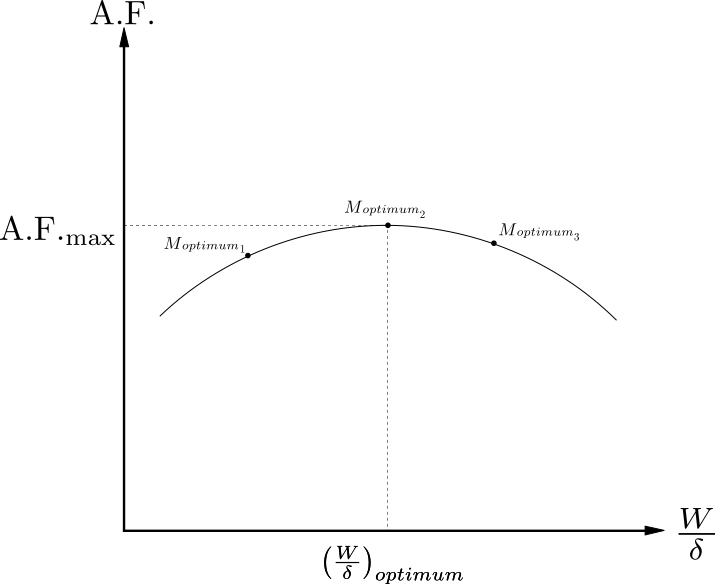
\includegraphics[keepaspectratio, width=0.60\textwidth]{AutonomyFactor}
\caption{Autonomy factor trend as function of the generalized weight}
\label{fig:Figure5}
\end{figure}

\noindent
As can be seen from figure~\ref{fig:Figure5} the autonomy factor has a maximum at a specific generalized weight which is the one that the pilot should maintain during the cruise phase. 

If the altitude is fixed, and so $\delta$ is constant, the chart in figure~\ref{fig:Figure5} can be seen as function of Mach number for a given aircraft weight; at this point, knowing that the autonomy factor leads to the specific range if divided by the aircraft weight, it's possible to define the specific range trend as funcion of the Mach number parameterized in aircraft weight. 

\begin{figure}[b]
\centering
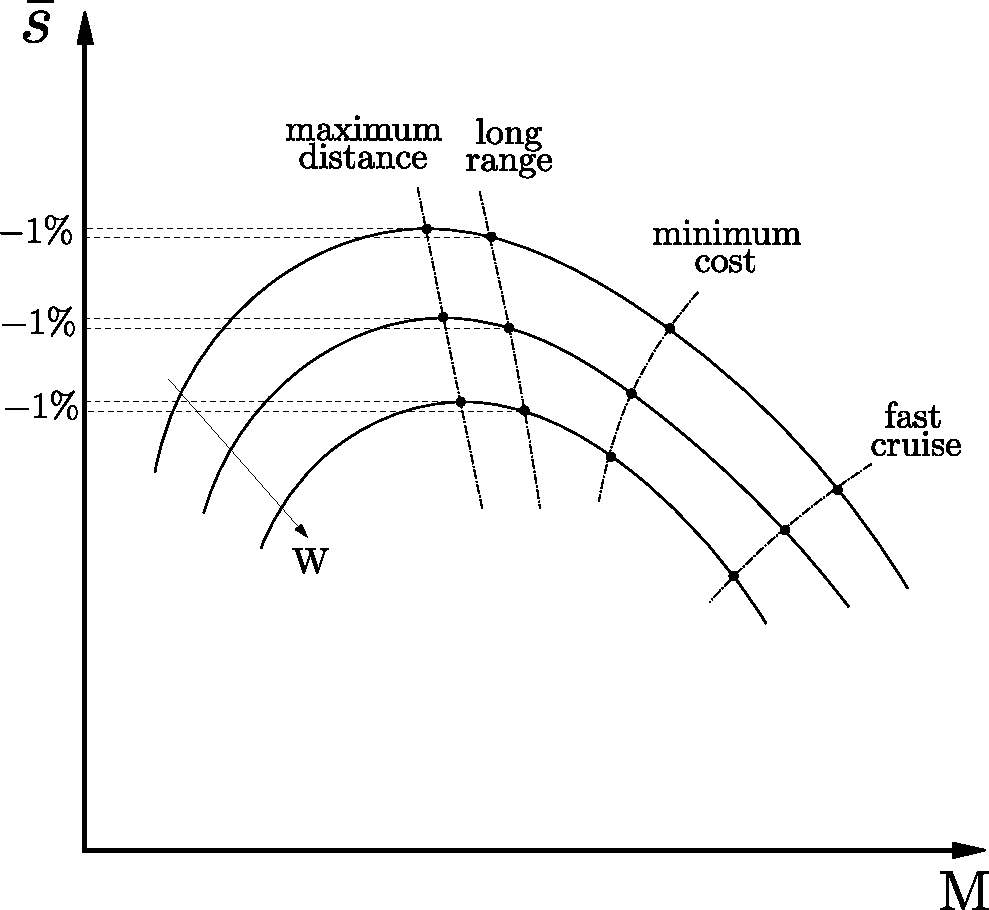
\includegraphics[keepaspectratio, width=0.50\textwidth]{CruiseGrid}
\caption{Specific range as function of the Mach number parameterized in aricraft weight}
\label{fig:Figure6}
\end{figure}

\bigskip
\noindent
The chart so obtained in figure~\ref{fig:Figure6} is the one upon which the cruise grid is defined; on the latter, in fact, four lines are drawn each of which is related to a precise mission objecive.

It's important to highlight that, on long distances, the maximum distance line is not often followed during the cruise because it is tied to a low speed which adversely affects the total flight time increasing the D.O.C.; in order to avoid this condition, pilots prefer to follow the long range line which has only 1\% of penalty on the specific range but, at the same time, allows to fly at significantly higher speed with benefits on flight time and, as a result, on the~D.O.C.

%------------------------- JAVA CLASS ARCHITECTURE ---------------------------
\section{Java class architecture}


%----------------------- CASE STUDY : ATR72 AND B747 -------------------------
\section{Case study: ATR-72 and B747-100B}
